\documentclass[12pt]{article}
\pdfoutput=1

\usepackage[OT1]{fontenc}
\usepackage[colorlinks,citecolor=blue,urlcolor=blue]{hyperref}
\usepackage[pdftex]{graphicx}
\usepackage{subfig}
\usepackage{fullpage}
\usepackage{palatino}
\usepackage{mathpazo}
\usepackage{amsmath}
\usepackage{amssymb}
\usepackage{color}
\usepackage{todonotes}
\usepackage{listings}

\usepackage[mmddyyyy,hhmmss]{datetime}

\definecolor{verbgray}{gray}{0.9}
\lstnewenvironment{csv}{%
  \lstset{backgroundcolor=\color{verbgray},
  frame=single,
  framerule=0pt,
  basicstyle=\ttfamily,
  columns=fullflexible}}{}

\begin{document}
  \begin{center}
		{\Large Practical 1: Predicting the Efficiency of Organic Photovoltaics}
		Camelot submission closes at 11:59pm on Thursday, February 8th, 2018\\
		Writeup due 11:59pm on Friday, February 9th 2018 
	\end{center}

	\bigskip
	
	\noindent You will do this assignment in groups of three. You can seek partners via Piazza. Course staff can also help you find partners. Please see \texttt{practical-logistics.pdf} for a description
    of competing on \href{https://portal.camelot.ai}{Camelot.ai}, what to submit to Canvas, and more. Make sure to use the provided \LaTeX \hspace{1pt} template for your writeup.
	
	
	\subsection*{The Harvard Clean Energy Project}
	
	\begin{quote}
		\emph{What if you could capture and convert sunlight into electricity with a material as cheap and as versatile as a plastic bag? What if the material could be produced on a massive scale, with easily accessible technology? What if other versions of the material could be coated, painted, or sprayed on building surfaces for solar energy production? What if these materials were ultra-thin and ultra-light for portable devices? And finally, what if they were inexpensive and could provide electricity to people in the developing world?} -- Harvard Clean Energy Project
	\end{quote}
	
	Solar power is one of the most promising technologies for renewable energy to reduce our dependence on fossil fuels.  Unfortunately, most modern solar cells are based on silicon.  These materials are rigid, expensive, and difficult to manufacture.  On the other hand, \emph{carbon} based solar cells could be cheap to produce, flexible, transparent, and be made and molded as easily as plastics.  There's just one catch: no known organic photovoltaic molecules are as efficient as their silicon counterparts.
	
	The Harvard Clean Energy Project has been using massive scales of computation to explore new possibilities for organic photovoltaics.  The project uses density functional theory (DFT) to estimate the the properties of the molecules that determine their potential efficiency as solar cells.  The main quantity of interest is the difference in energy between the highest occupied molecular orbital (HOMO) and the lowest unoccupied molecular orbital (LUMO).  It can take hours or days to compute this accurately on a modern computer.
	
	Recently, it has become clear that machine learning might have something to say about this.  It may be possible to sidestep these expensive DFT computations by learning a function from a feature representation of the molecule to the HOMO-LUMO gap.  From our point of view in CS181, this is a regression problem: take molecular features and produce a real-valued prediction of what the DFT would calculate.  Better machine learning models for this problem could lead to new kind of materials and more efficient solar cells!
	
	You have one million molecules to train on, and are tasked with making predictions on another 800,000 or so.  You'll upload your predictions to Camelot, where a subset will be used to produce a ``public leaderboard'' and another subset will be used to reveal the final rankings at the end of the contest.  You'll have access to complete information about the molecular structure in the form of a SMILES string.  This is a representation that chemists like to use to encode molecular structures.  Here is an example:
	\begin{center}
		c1sc(-c2sc(-c3ccc(cc3)-c3scc4sccc34)c3[se]ccc23)c2sccc12
	\end{center}
	This SMILES string is a molecule that looks like this:
	\begin{center}
		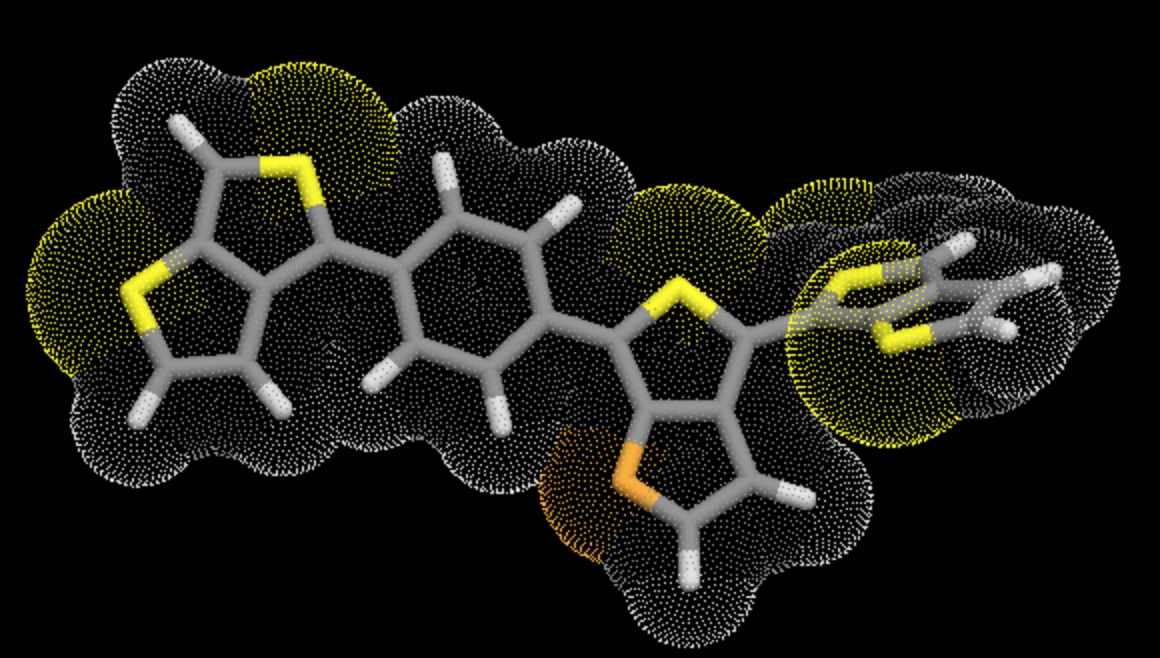
\includegraphics[width=3in]{molecule}
	\end{center}
	
	One of the challenges of making predictions about molecules is finding a good feature representation.  Clearly, the SMILES string itself isn't going to be all that helpful.  Luckily, many chemists have built tools to build interesting representations.  One such tool is a Python package called \href{http://www.rdkit.org/}{RDKit}.  With it you can easily load SMILES strings and produce features. Alternatively, you can just use the features we've already extracted with RDKit, which produced 256-dimensional binary vectors.  These vectors are in the training and test files provided.
	
	\subsection*{Data Files}
	There are five files of interest, which you can get from the \href{https://github.com/harvard-ml-courses/cs181-s18-practicals/tree/master/P1}{Github repository}. 
	\begin{itemize}
		\item \verb|train.csv.gz| -- This file contains information about one million molecules.  It has 258 columns.  The first column is a SMILES string, which is a representation of the molecule in case you would like to see what it looks like or build better feature representations. The next 256 columns are a binary feature representation that RDKit outputs.  These are features of the molecule that you might use to build a regression model.  The final column is the difference in energy between the HOMO and the LUMO.  This is the label you are trying to predict.
		\item \verb|test.csv.gz| -- This file contains another 800,000 or so molecules.  In this case, the label is not provided.  These are the ones you are trying to make predictions for. The first column is a numeric identifier that you should use when constructing your prediction file to upload to Camelot.
		\item \verb|sample.ipynb| -- This is a simple IPython notebook that produces the predictive files \verb|sample1.csv| and \verb|sample2.csv|.  Feel free to build off of this notebook.
		\item \verb|sample1.csv| -- This is an example of a prediction file you might upload to Camelot.  The id numbers match those in the test file, but the predictions are very na\"ive: just the untuned outputs of linear regression produced by \verb|sample.ipynb|.
		\item \verb|sample2.csv| -- This is an example of a prediction file you might upload to Camelot.  The id numbers match those in the test file, but the predictions are very na\"ive: just the untuned outputs of random forests regression produced by \verb|sample.ipynb|.
	\end{itemize}
	
	\subsection*{Evaluation}
	After you upload your predictions to Camelot (which you can do at most four times per day), they will be compared to the held-out true HOMO-LUMO gaps, as determined by density functional theory calculations.  The score is computed via root mean squared error (lower is better).  If there are~$N$ test data, where your prediction is~$\hat{x}_n$ and the truth is~$x_n$, then the RMSE is 
	\begin{align*}
		\text{RMSE} &= \sqrt{\frac{1}{N}\sum_{n=1}^N (\hat{x}_n-x_n)^2}
	\end{align*}
	
	\subsection*{Sample Code}
	An IPython notebook is available from the course website to help you get going.  The file called \verb|sample.ipynb| is a simple script to load in data and produce the \verb|sample1.csv| and \verb|sample2.csv| prediction files.  You don't need to use this file; feel free to build the prediction system as you see fit.
	
	\subsection*{Sample Baselines}
	On the Camelot leaderboard, there are two baseline scores.  One determined by Linear Regression and the other determined by Random Forest Regression on \textit{just} the default data -- no feature engineering or parameter tuning.  To see how these scores were obtained, take a look at \verb|sample.ipynb|.  To earn full points, you must achieve a score higher than both.  Remember, the public leaderboard will only display a fraction of the \textit{entire} test set, so scores may drastically change if you overfit!  After the Camelot submission closes, the scores on the full test set will be computed and shown.  We will be going off the final scores. 
	\textbf{Hint: Minor feature engineering, i.e., adding on more features will graciously better your score!}  Don't just use the default data.  Be creative!
	
	\subsection*{Solution Ideas}  You have a lot of flexibility in what you might do.  You could focus on feature engineering, i.e., coming up with fancy inputs for your method using a tool like RDKit (or your own knowledge of chemistry!), or you could focus on fancy regression techniques that use the features we provide. We encourage that you use the sklearn package from Python when building your models.  Here are some ideas to get you started:
	\begin{itemize}
		
		\item \textbf{Ridge Regression:} You could use a simple $L_2$ regularization approach to regression weights and use cross-validation to determine an appropriate regularization penalty.
		\item \textbf{Lasso Regression:} You could got a bit fancier and use $L_1$ regression to identify a sparse solution, again using cross-validation to determine an appropriate regularization penalty.
		\item \textbf{Elastic Net:} Use both $L_1$ and $L_2$ at once!
		\item \textbf{Neural Network:} Get a jump on the course material and build a neural network to make predictions.  Explore the world of deep learning!
		\item \textbf{Ensemble Methods:}
		Want to be robust?  Use bootstrap aggregation with decision tree learning! 
		\item \textbf{Support Vector Regression:} Prefer your problem convex? Get a jump on kernel methods and build a support vector machine for regression.
		\item \textbf{New Feature Ideas:} Try out some of the different fancy feature representations and chemical fingerprints that different cheminformatics tools provide.  Maybe there's even a better way to use RDKit to extract features.
		\item \textbf{Go Totally Bayesian:} Worried that you're not accounting for uncertainty?  You could take a fully Bayesian approach to linear regression and marginalize out your uncertainty.
		\item \textbf{Go Nonparametric Bayesian:} Intrigued by the infinite-dimensional machine learning?  Check out \href{http://www.gaussianprocess.org/gpml/}{Gaussian process regression}.
		
	\end{itemize}
	
	
	
\end{document}
